\documentclass[conference]{IEEEtran}
\IEEEoverridecommandlockouts
% The preceding line is only needed to identify funding in the first footnote. If that is unneeded, please comment it out.
\usepackage{cite}
\usepackage{amsmath,amssymb,amsfonts}
\usepackage{algorithmic}
\usepackage{graphicx}
\graphicspath{{figures/}}
\usepackage{textcomp}
\usepackage{xcolor}
\usepackage{listings}
\usepackage[breaklinks=true, hidelinks]{hyperref}

\lstset{
  language=C,
  basicstyle=\ttfamily\scriptsize,
  keywordstyle=\color{blue}\bfseries,
  stringstyle=\color{red},
  commentstyle=\color{green!60!black},
  numbers=left,
  numberstyle=\tiny\color{gray},
  stepnumber=1,
  breaklines=true,
  breakatwhitespace=true,
  tabsize=2,
  captionpos=b,
  frame=lines
}

\def\BibTeX{{\rm B\kern-.05em{\sc i\kern-.025em b}\kern-.08em
    T\kern-.1667em\lower.7ex\hbox{E}\kern-.125emX}}
    
\begin{document}

\title{Real-Time Light Dosimetry for Heritage Digital Twins via Texture Space Ray Tracing}

\author{\IEEEauthorblockN{Sebastian Duică}
    \IEEEauthorblockA{\textit{Computer Science Department} \\
        \textit{Technical University of Cluj-Napoca}\\
        Cluj-Napoca, Romania \\
        Duica.Ro.Sebastian@student.utcluj.ro} \\
    % \and
    % \IEEEauthorblockN{Advisor Name}
    % \IEEEauthorblockA{\textit{Computer Science Department} \\
    % \textit{Technical University of Cluj-Napoca}\\
    % Cluj-Napoca, Romania \\
    % advisor.email@example.com}
}

\maketitle

\begin{abstract}
    Light damage dosimetry is essential for preserving cultural heritage and avoiding permanent photochemical degradation. Modern approaches to simulation of light dosimetry employ computationally heavy off-line software lacking in interactivity; thus, planning processes are hindered. In order to overcome such difficulties, ChronoLux, an innovative Digital Twin solution using Texture Space Ray Tracing technique for interactive light dosimetry is proposed. Instead of utilizing conventional screen-space algorithms that do not incorporate physical information on the temporal changes in energy into the UV-map of the artefact, ChronoLux offers real-time editing of architectural materials and artifact positioning. Moreover, apart from interactivity, the proposed approach provides instant results regarding dose variation over the surface of the object. Results of a year-long simulation prove that the framework produces metrologically precise information despite being fully interactive: with proper environmental adjustments, peak dose per annum dropped from 6.6 M to less than 150 kLux-Hours without disturbing Monte Carlo sensor convergence.
\end{abstract}

\begin{IEEEkeywords}
    Digital Twins, Cultural Heritage, Ray Tracing, Light Dosimetry, Monte Carlo Integration, GPU Acceleration, DXR
\end{IEEEkeywords}

\section{Introduction}

Light dosimetry is the calculation of radiative energy (in Lux-Hours) incident upon the surface during a certain amount of time period. The calculation is required for the conservation of cultural heritage where museum curators want to protect artifacts from light exposure and excessive heating.

Traditionally, such type of prediction was performed using some generalized models of lighting and/or off-line architectural rendering solutions. The problem with these approaches is that due to being off-line, rendering-based approaches, they prevent the possibility to evaluate the influence of window glazing changes, materials of the rooms and objects themselves, and so forth in real time. To fill this gap, the authors propose to use the concept of Digital Twin to estimate light doses interactively. In other words, unlike camera-to-image ray casting approach used by many existing tools, the new technique uses a texture space ray tracing when texture coordinates are used to cast rays and produce realistic irradiance values. When combined with the Perez all-weather sky model and NEE, both ambient and direct irradiation can be estimated interactively. Furthermore, the concept of Digital Twin allows performing the process of irradiance values accumulation independently of a certain screen space or camera position.

The other innovation brought by the authors is the possibility of virtual point-probe sensor implementation and thus, evaluation of the error of the Monte-Carlo method. According to the experimental results obtained in the course of 2k-resolution textured 3D artifact modeling through the year, the proposed approach managed to reduce significantly the structural contrast stress reaching end-of-the year peak value reduction of 97.7\%.

\section{Related Work}

\subsection{Physical Dosimetry and IoT Sensor Networks}

In terms of the real-world application of preventive conservation practices in museums, there has been a clear shift towards utilizing IoCT and physical light dosimetry approaches. The latest generation of IoT photometers \cite{silva2020climate} allows for continual and remote monitoring of the levels of ambient light, thereby enabling the relevant museum personnel to take action once light exposure surpasses acceptable limits \cite{chianese2016internet}. Physical photometric measurements can be used for obtaining ground truth, but such devices exhibit two main shortcomings, being merely reactive and measuring irradiance at just one localized point. ChronoLux complements physical photometers by providing the ability to simulate spatial dose variation throughout the artifact geometry continuously.

\subsection{Traditional Simulation in Conservation}

In the case of predictive analysis, the typical process involves extensive use of offline architectural simulation software packages, such as Radiance \cite{ward1998rendering}. Utilizing backward ray-tracing algorithms and irradiance caching, such tools offer a reliable approach for accurately modeling the physical lighting distributions in architectural geometry. However, they are frequently employed in the calculation of lighting limits according to preventive conservation guidelines defined by Michalski \cite{michalski1987damage} and the International Commission on Illumination (CIE) \cite{cie2004control}, where museum exhibits should be exposed for no more than certain numbers of Lux-Hours per year (e.g., no more than 50,000 Lux-Hours for highly sensitive materials like watercolor or textile paintings). While the offline simulation ensures an extremely precise, mathematically provable physical model and lighting distribution calculations, its very architecture imposes a significant bottleneck in the conservation workflow. In particular, lacking a hardware-accelerated renderer with real-time denoising and being limited to CPU-only calculations, the calculation of a single, one-year long exposure with hourly resolution might take up to several hours, thus prohibiting any sort of interactive work with the data. As opposed to those traditional simulators, ChronoLux provides the same level of physically accurate metrology, i.e., respects Lambertian scattering and energy conservation laws, but at real-time render speeds using a GPU-powered approach.

\subsection{Precomputed Illumination in Virtual Heritage}

In order to overcome the processing limitations of offline rendering, many virtual heritage projects use Precomputed Radiance Transfer (PRT) along with lightmaps to enable interactive frame rates \cite{sloan2002precomputed}. This enables exploration of heritage assets with physically accurate lighting that is computed offline and hence not interactive. Inherently, PRT works under the assumption of a static scene. Should one wish to modify the transmittance values of the conservation glass or alter the position of the asset for testing purposes, the lightmap will need to be re-computed again from scratch, defeating the very purpose of interactivity.

\subsection{Advances in Real-Time Ray Tracing}

The adoption of hardware-accelerated Monte Carlo Path Tracing methods \cite{kajiya1986rendering, veach1995optimally} using the latest generation of Direct X Ray Tracing architecture \cite{burgess2020rtx} marks a milestone in the field of interactive graphics. The existence of dedicated hardware cores designed for BVH traversal and ray intersection has made real-time Global Illumination possible. This trend is accompanied by the rise of Texture Space Shading (TSS) \cite{hasselgren2016texture}, which allows us to remove shading from the pixel grid of the final image. Most recently, TSS technology has gained the ability to cache and stabilize Monte Carlo noise between temporal frames \cite{smith2024texture}, making it possible to use cached shading results between frames and implement complicated materials without temporal aliasing. Nonetheless, despite these breakthroughs in the technology, all existing frameworks of real-time ray-tracing remain optimized mostly for visual performance and screen-space frame rate. These systems discard the lighting information outside the bounds of the camera's view using the frustum culling approach and don't support persistence in accumulations of raw Lux-Hours over time. ChronoLux is a framework that re-architects this DXR pipeline and uses ray launches from texture space coordinates instead of the virtual camera lenses to make the process of shading completely mathematically sound and independent of the camera itself.

\subsection{Digital Twins in Cultural Heritage}

Digital Twins are now more commonly being applied in the digitization process of heritage assets using 3D laser scanning technologies \cite{niccolucci2022digital, jouan2020digital}. With all the developments, many heritage digital twins continue to be used merely as informative databases or as sensor alert mechanisms that operate reactively instead of predictively through simulation. This is where ChronoLux comes in. This approach converts passive 3D models into virtual simulations governed by the Perez All-Weather Sky Model \cite{perez1993all} and leveraging modern hardware for maximum accuracy and performance.

\section{Methodology \& System Architecture}

The architecture of ChronoLux is described in more detail below in terms of system components, numerical methods and GPU accelerated render paradigms employed. Figure~\ref{fig:architecture} demonstrates how the application operates as an advanced Digital Twin running inside a modern C\#/DirectX 12 graphics engine. The proposed architecture strictly separates the UI layer based on UXML/USS frameworks for controlling material properties of reflectance and transmittance and physics simulation layer. In contrast to traditional approaches, the innovation introduced by our solution is the transition from transient screen space rendering to permanent Texture Space Ray Tracing method, which enables rigorous accumulation of radiometric data across full 8760 hours of meteorological years, followed by extraction by a dedicated headless C\# telemetry module for statistical analysis.

The ability to serialize the scene using an effective engine is crucial for the viability of the framework as a Persistent Digital Twin. Not only does the UI manage the interactive material library and solar data feed, but it automatically persists all changes made to objects, such as translations and scaling, as well as material assignment in terms of reflectivity and transmissiveness, on a submesh level. This process of seamless persistence allows any experimental setup, including those architectural modifications tested in our experiments, to persist indefinitely, without any loss of fidelity.

\begin{figure*}[t]
    \centerline{
\includegraphics[width=0.8\textwidth]{architecture.png}}
    \caption{High-level system architecture of ChronoLux, demonstrating the decoupled data flow from the UXML UI layer to the DX12 GPU Compute Pipeline, culminating in persistent CSV/EXR storage.}
    \label{fig:architecture}
\end{figure*}

\subsection{The Physics of Light Dosimetry}

In order to simulate photo-degradation of historical artifacts properly, it is necessary to create a mathematically rigorous model of light exposure. Traditional conservator methods consider the amount of light falling on an object (irradiance) as an integral of incoming radiance, projected along the incident angle using Lambert's Cosine Law:
\begin{equation}
    E = \int_{\Omega} L_i(\omega_i) \cdot \cos(\theta) \, d\omega_i
\end{equation}
ChronoLux framework applies a discrete approximation of the above-mentioned integration process via summing up all hourly exposures within a full meteorological year of 8760 hours: $D_{total} \approx \sum_{t=1}^{8760} E(t) \cdot \Delta t$. In order to provide physically sound energy conservation and inter-reflections of light rays within the environment, all architectural materials in the environment have the constraint on the sum of reflectance ($R$) and transmittance ($T$): $R + T \le 1.0$. The above-mentioned mathematical rigor guarantees that radiometric data exported from the Digital Twin will be perfectly aligned with established scientific recommendations \cite{cie2004control} and would serve as a solid basis for further action by the curator instead of meaningless pixel values.

\subsection{Texture Space Ray Tracing Architecture}

One of the fundamental limitations of the current HW accelerated ray tracing framework such as DirectX 12 is its dependence on screen space rendering. In traditional game engine architecture, a special type of camera is used, where rays are casted outward to represent visible pixels. As a result, anything lying outside the field of view of the camera is simply clipped away. This approach is completely unacceptable in the context of scientific light dosimetries where the continuous irradiance measurement of the whole geometrical surface is mandatory regardless of where exactly the user is looking. In order to overcome this limitation, the ChronoLux framework re-architects the DXR pipeline into Texture Space.

\begin{figure}[htbp]
    \centerline{
\includegraphics[width=\columnwidth]{pipeline.png}}
    \caption{The Texture Space Ray Tracing pipeline. The architecture bypasses the camera by pre-computing UV Position/Normal maps, allowing the compute shader to launch rays directly from the artifact's surface.}
    \label{fig:pipeline}
\end{figure}

In brief, given an input 3D model, the framework runs special UV baker pre-pass where UV map is calculated. At this stage, the system also produces special RenderTexture in \texttt{RGBFloat} format storing Position and Normal coordinates in world space at every texel. Careful attention is paid to the fact that Z-clipping in this prepass must be set to $Z = 0.5$ as well as inversion of Y axis in order to conform to DirectX12 texture coordinates requirements. Finally, the core Ray Tracing Compute Shader is called in a way that makes its every thread to correspond to particular UV texel. As a consequence, every millimeter of the 3D model surface is independently calculating lighting conditions.

\begin{figure}[htbp]
    \begin{algorithmic}
        \REQUIRE $PosMap, NormMap, SunDir, N_{samples}, \Delta t$
        \FOR{\textbf{each} thread $id \in \text{DispatchThreadID}$}
        \STATE $\mathbf{p} \leftarrow PosMap[id].xyz$
        \STATE $\mathbf{n} \leftarrow NormMap[id].xyz$
        \IF{$||\mathbf{n}|| < 0.1$}
        \STATE \textbf{return}
        \ENDIF
        \STATE $E_{dir} \leftarrow \textsc{TraceShadow}(\mathbf{p}, SunDir) \cdot \max(0, \mathbf{n} \cdot SunDir)$
        \STATE $E_{ind} \leftarrow 0$
        \FOR{$i = 1$ \textbf{to} $N_{samples}$}
        \STATE $\omega_i \leftarrow \textsc{SampleCosineHemisphere}(\mathbf{n})$
        \STATE $E_{ind} \leftarrow E_{ind} + \textsc{TracePerezSky}(\mathbf{p}, \omega_i)$
        \ENDFOR
        \STATE $E_{total} \leftarrow E_{dir} + (E_{ind} / N_{samples}) \cdot \pi$
        \STATE $DoseMap[id] \leftarrow DoseMap[id] + E_{total} \cdot \Delta t$
        \ENDFOR
    \end{algorithmic}
    \caption{Pseudocode for Texture Space Ray Tracing Algorithm}
    \label{alg:ts_raytrace}
\end{figure}

As it is shown in Algorithm~\ref{alg:ts_raytrace}, the proposed architecture makes the process of light simulation completely detached from screen space thus ensuring permanent bake down of energy data into the texture map. Thus, a very convenient irradiance accumulator is implemented which permanently maps thermal and light stress onto the geometry surface.

\subsection{Environmental Modeling and NEE}

Calculating cumulative impact of irradiance requires simulation of the whole spectrum of light ranging from ambient skylight illumination to direct sunlight radiation throughout one meteorological year. Static single directional light source cannot properly represent the dynamic shadow behavior created by moving windows or changing position of the sun. To solve this issue, ChronoLux incorporates Perez All-Weather Sky Model \cite{perez1993all} that computes precise sky luminance values according to real world climatic conditions and solar altitude.

During the ray generation kernel, the framework uses Next Event Estimation technique (NEE) by leveraging Monte Carlo path tracing algorithm to converge faster. In particular, in every UV texel shader performs separation of the rendering integral into two parts. Firstly, it casts the shadow ray pointing directly to localized solar disc and computes the irradiance, taking account of any architectural occlusions. Secondly, it performs a weighted sample cosine distribution across hemisphere in order to accumulate diffuse ambient skylight irradiance according to Perez distribution. Such an approach makes it possible to simulate complex high frequency architectural shadows, while not introducing additional Monte Carlo noise and not forcing us to use a large number of samples.

\subsection{Statistical Metrology \& Data Telemetry}

Despite the fact that heat map visualization (with consideration of the Inferno color palette) provides valuable information for the qualitative assessment of the scene, it cannot be used to publish any results or provide scientific information needed for the purposes of conservation. Therefore, the quantitative availability of the information about light dose becomes critical in terms of statistical analysis. While the visualization allows us to identify problem areas on the scene, it does not provide enough information to confirm the presence of problems and take appropriate measures. For this reason, the idea of placing virtual Lux Sensors outside the scene was implemented. They allow for automatic positioning of control probes and extraction of the telemetry data right from the accumulation buffer without tonemapping. At this stage, we can start analyzing such data as:

\begin{equation}
    \sigma^2 = \frac{1}{N} \sum_{i=1}^{N} (D_i - \bar{D})^2
\end{equation}
Furthermore, these virtual Lux probes calculate real time Monte Carlo convergence errors compared to theoretical values. Considering the fact that any attempt of GPU to CPU readout introduces serious synchronization issues, the telemetry process proceeds asynchronously utilizing a background headless thread in C\#. As detailed in Algorithm~\ref{alg:async_telemetry}, this thread safely sums up every hourly delta value as well as maximum exposure and variance metrics, exporting the results to a standard CSV array without interrupting the 60 FPS render cycle.

\begin{figure}[htbp]
    \begin{algorithmic}
        \REQUIRE $AccumBuf$, $CSVStream$, $CurrentHour$
        \STATE $\textsc{DispatchComputeShader}(CurrentHour)$
        \STATE $Request \leftarrow \textsc{AsyncGPUReadback}(AccumBuf)$
        \WHILE{\textbf{not} $Request.isDone$}
        \STATE \textbf{yield return} $\text{null} \quad \text{// Maintain 60 FPS render cycle}$
        \ENDWHILE
        \STATE $Data \leftarrow Request.\textsc{GetData}()$
        \STATE $\mu \leftarrow 0, \; MaxDose \leftarrow 0, \; \sigma^2 \leftarrow 0$
        \FOR{\textbf{each} $p \in Data$}
        \STATE $\mu \leftarrow \mu + (p / N)$
        \STATE $MaxDose \leftarrow \max(MaxDose, p)$
        \ENDFOR
        \FOR{\textbf{each} $p \in Data$}
        \STATE $\sigma^2 \leftarrow \sigma^2 + (p - \mu)^2 / N$
        \ENDFOR
        \STATE $CSVStream.\textsc{Append}(CurrentHour, MaxDose, \mu, \sigma^2)$
    \end{algorithmic}
    \caption{Asynchronous Headless Telemetry Extraction Pipeline}
    \label{alg:async_telemetry}
\end{figure}


\section{Case Studies \& Empirical Results}

\subsection{Experimental Setup \& Simulation Parameters}
For empirical validation of ChronoLux's ability to quantify light stress, a number of case study simulations were performed on a high-fidelity 3D scan of the Stanford Bunny, represented in 2K resolution UV textures. The virtual environment was located at Latitude 44.427, Longitude 26.103 (Bucharest, Romania), and the simulation calculated a series of discrete hourly solar intervals for the entire meteorological year 2026 (8760 hours). The ray-tracing engine was tuned to perform 64 Monte Carlo rays per UV texel.

An important detail about our approach is that the model for calculating sunlight used is the Perez All-Weather Sky Model configured with a static value of $T = 2.0$. This corresponds to a mathematical representation of clear sky with no clouds. Although real-life weather fluctuates, the perpetually clear sky assumption is used to make a deliberate meteorological choice to apply stress testing in the Digital Twin in the absolute worst case scenario, thereby guaranteeing that the conservation measures applied in this scenario can handle the strongest possible annual photodegradation forces.

\subsection{Scenario A: The Baseline Exposure}
Scenario A uses the baseline setup of the asset being situated in a highly exposed place next to a window. Architectural material properties were set to replicate untreated museum conditions: floor albedo $R = 0.50$, while windows were made from clear glass material with transmittance $T = 0.84$ and albedo $R = 0.08$.

This configuration presents a worst case baseline of unlimited light exposure to the asset.

\begin{figure}[htbp]
    \centerline{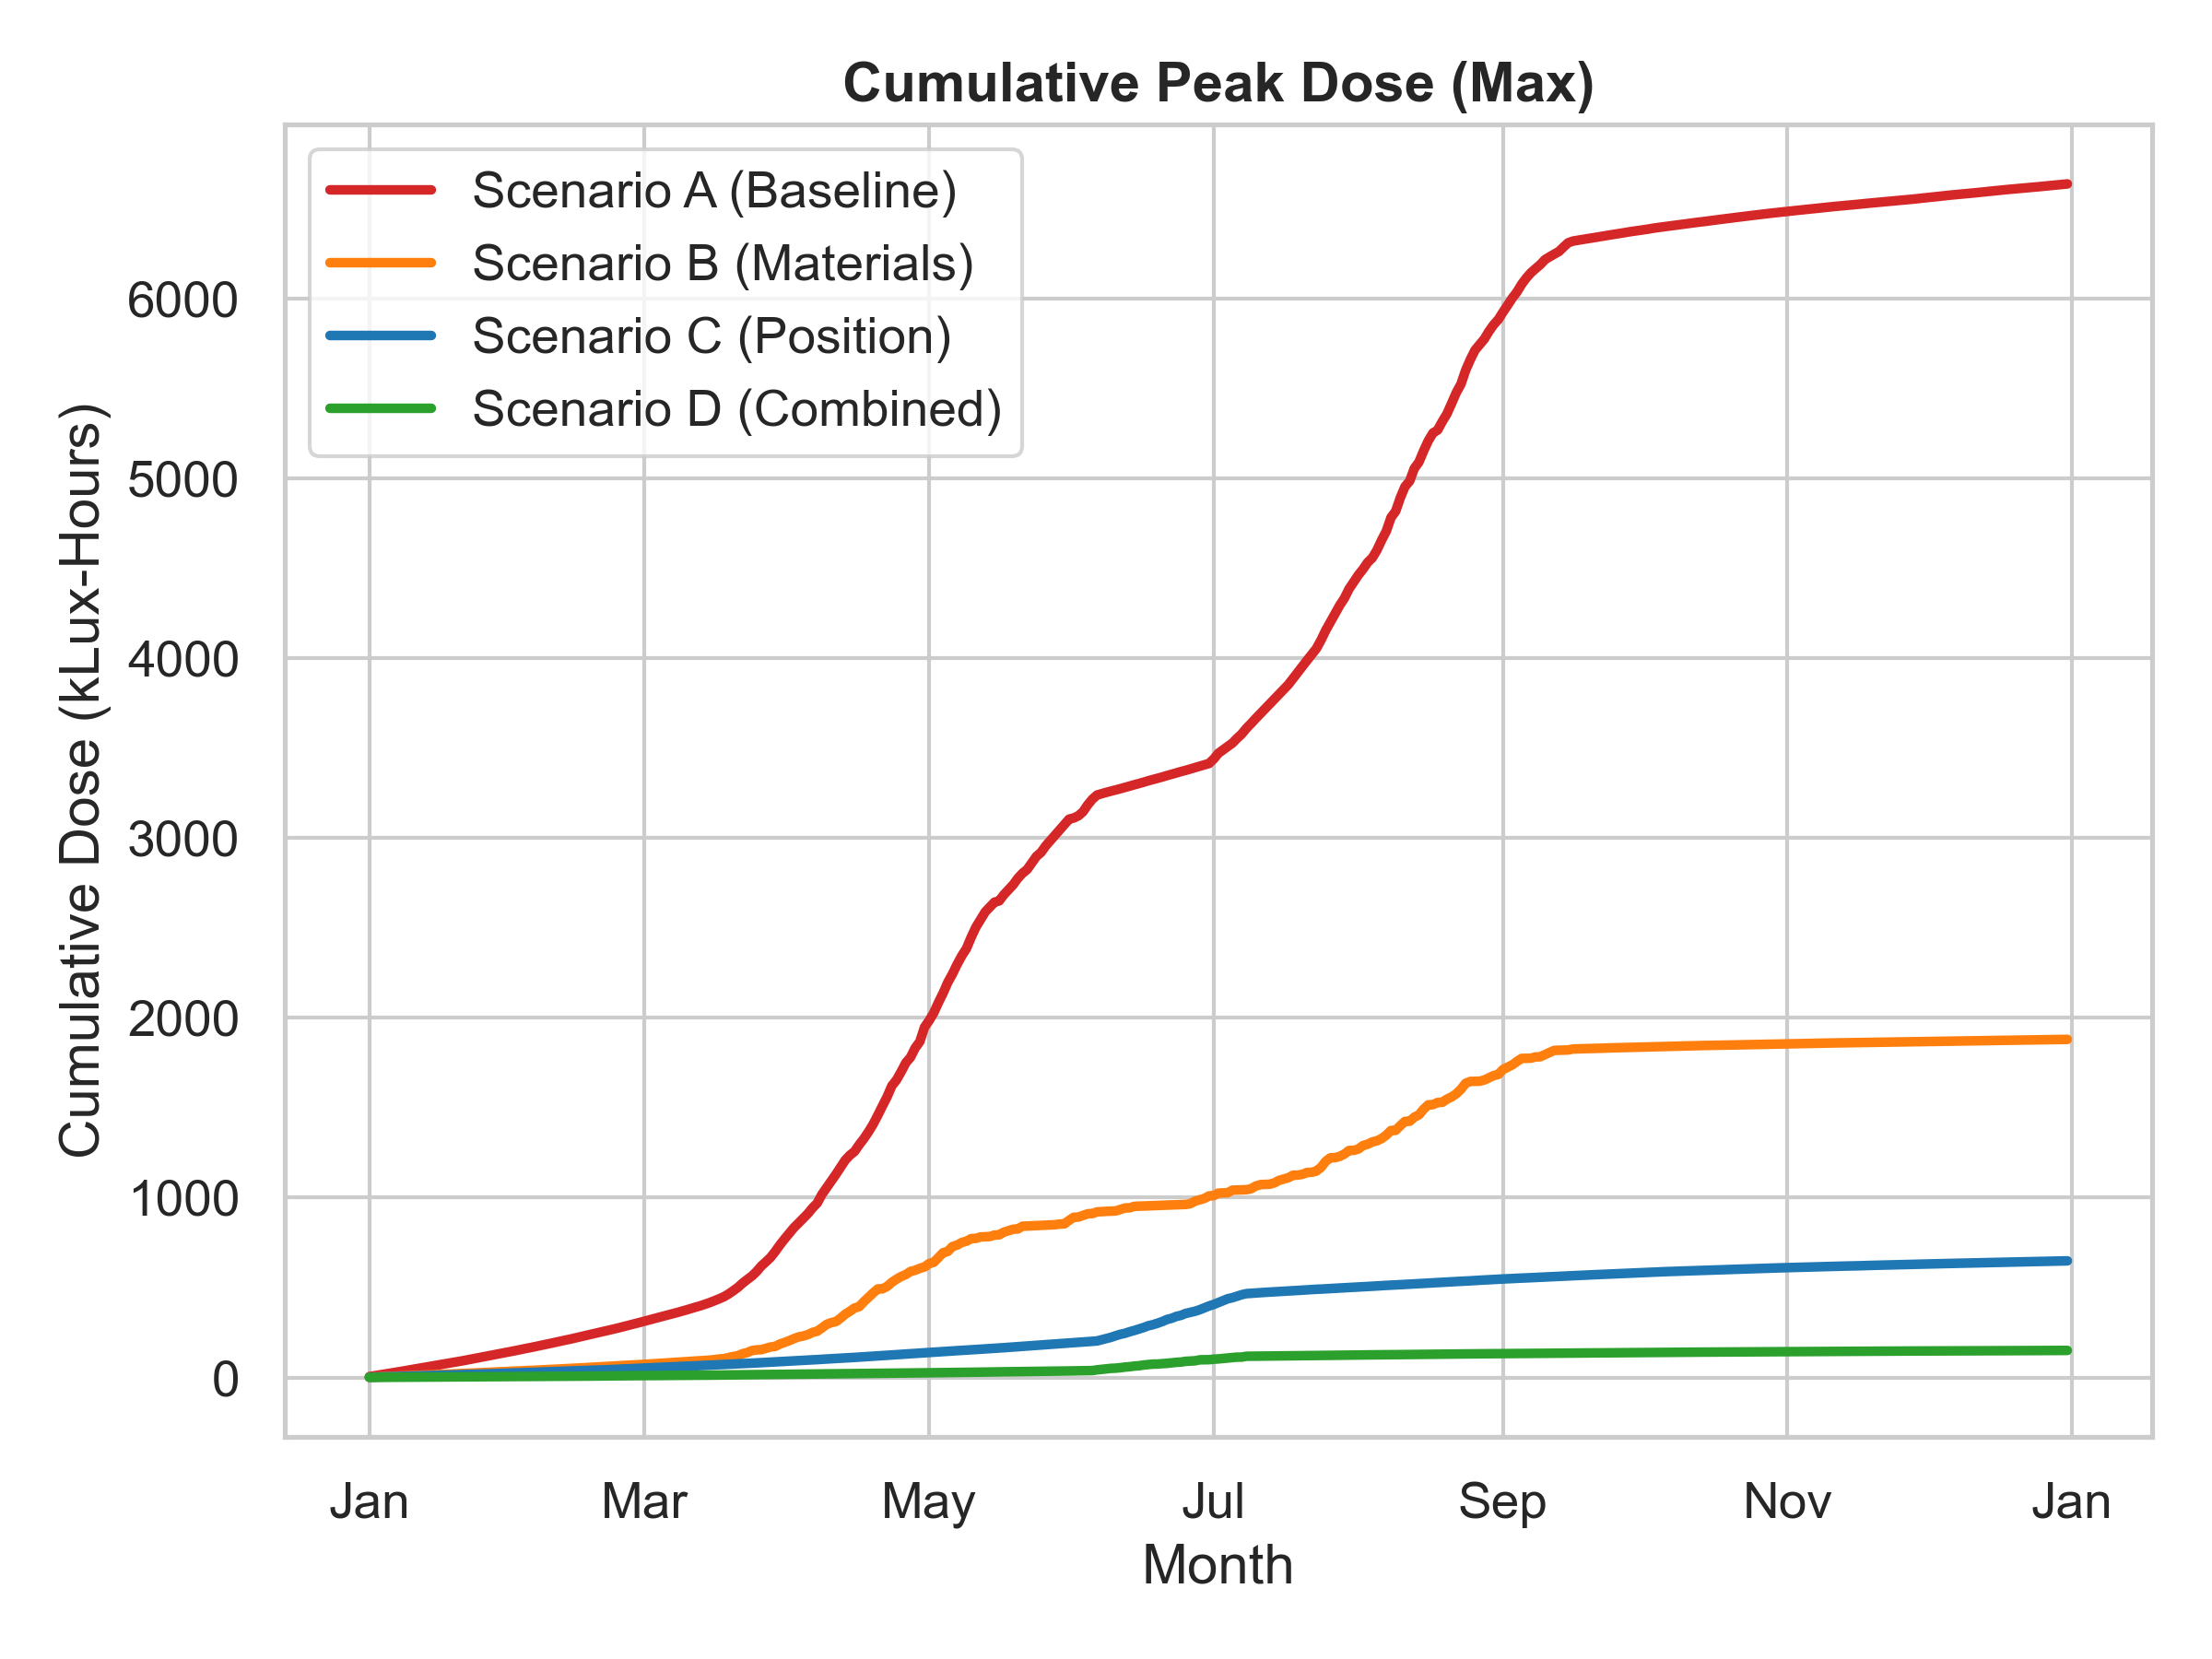
\includegraphics[width=0.9\columnwidth]{fig1a_cumulative_max_dose.png}}
    \caption{CIE Light Dosimetry results for Scenario A reveal cumulative light stress exposure over 8760 hours resulting in a large peak light dose of 6.6M Lux-Hours far greater than the maximum recommended light stress of 50,000 Lux-Hours.}
    \label{fig:scenario_a_max}
\end{figure}

\begin{figure}[htbp]
    \centerline{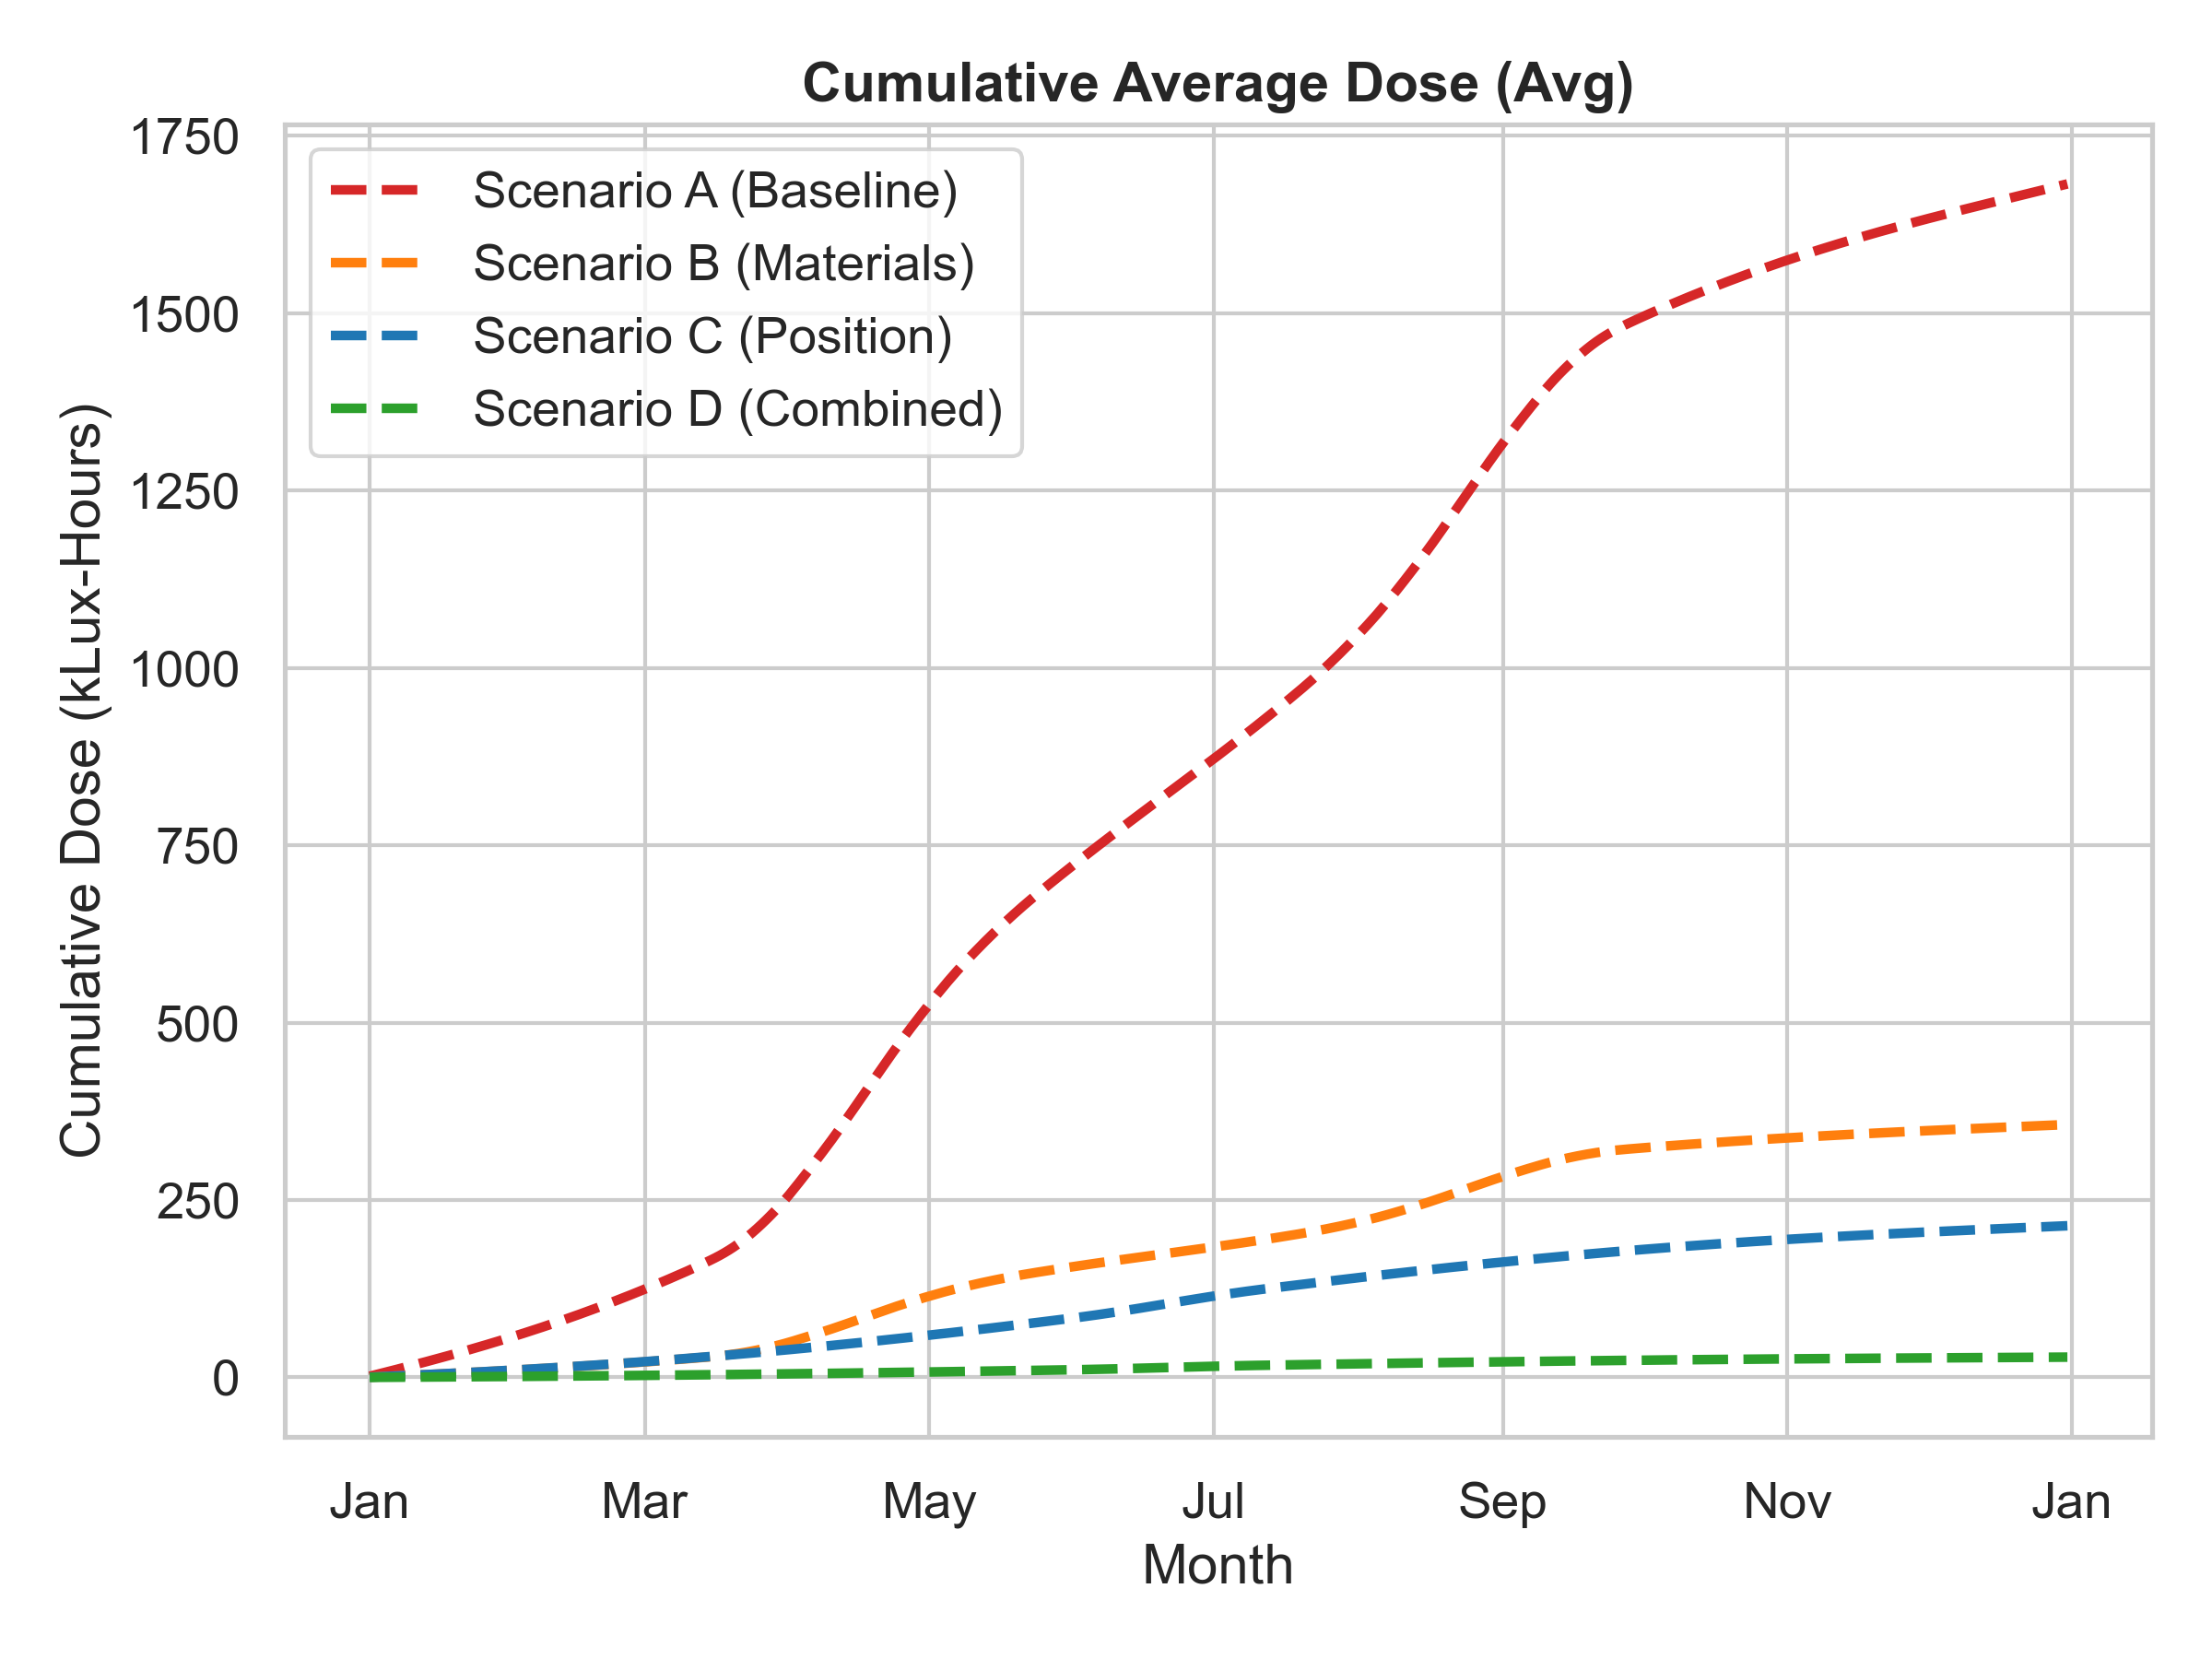
\includegraphics[width=0.9\columnwidth]{fig1b_cumulative_avg_dose.png}}
    \caption{CIE Light Dosimetry results for Scenario A showing cumulative average dose over the 8760 hours.}
    \label{fig:scenario_a_avg}
\end{figure}

As shown in Figure~\ref{fig:scenario_a_max} and Figure~\ref{fig:scenario_a_avg}, the result of such an extreme configuration is the catastrophic peak light dose of 6.6M Lux-Hours  far surpassing the maximum light stress capacity of CIE's recommended 50,000 Lux-Hour threshold for sensitive materials \cite{cie2004control}.

\begin{figure}[htbp]
    \centerline{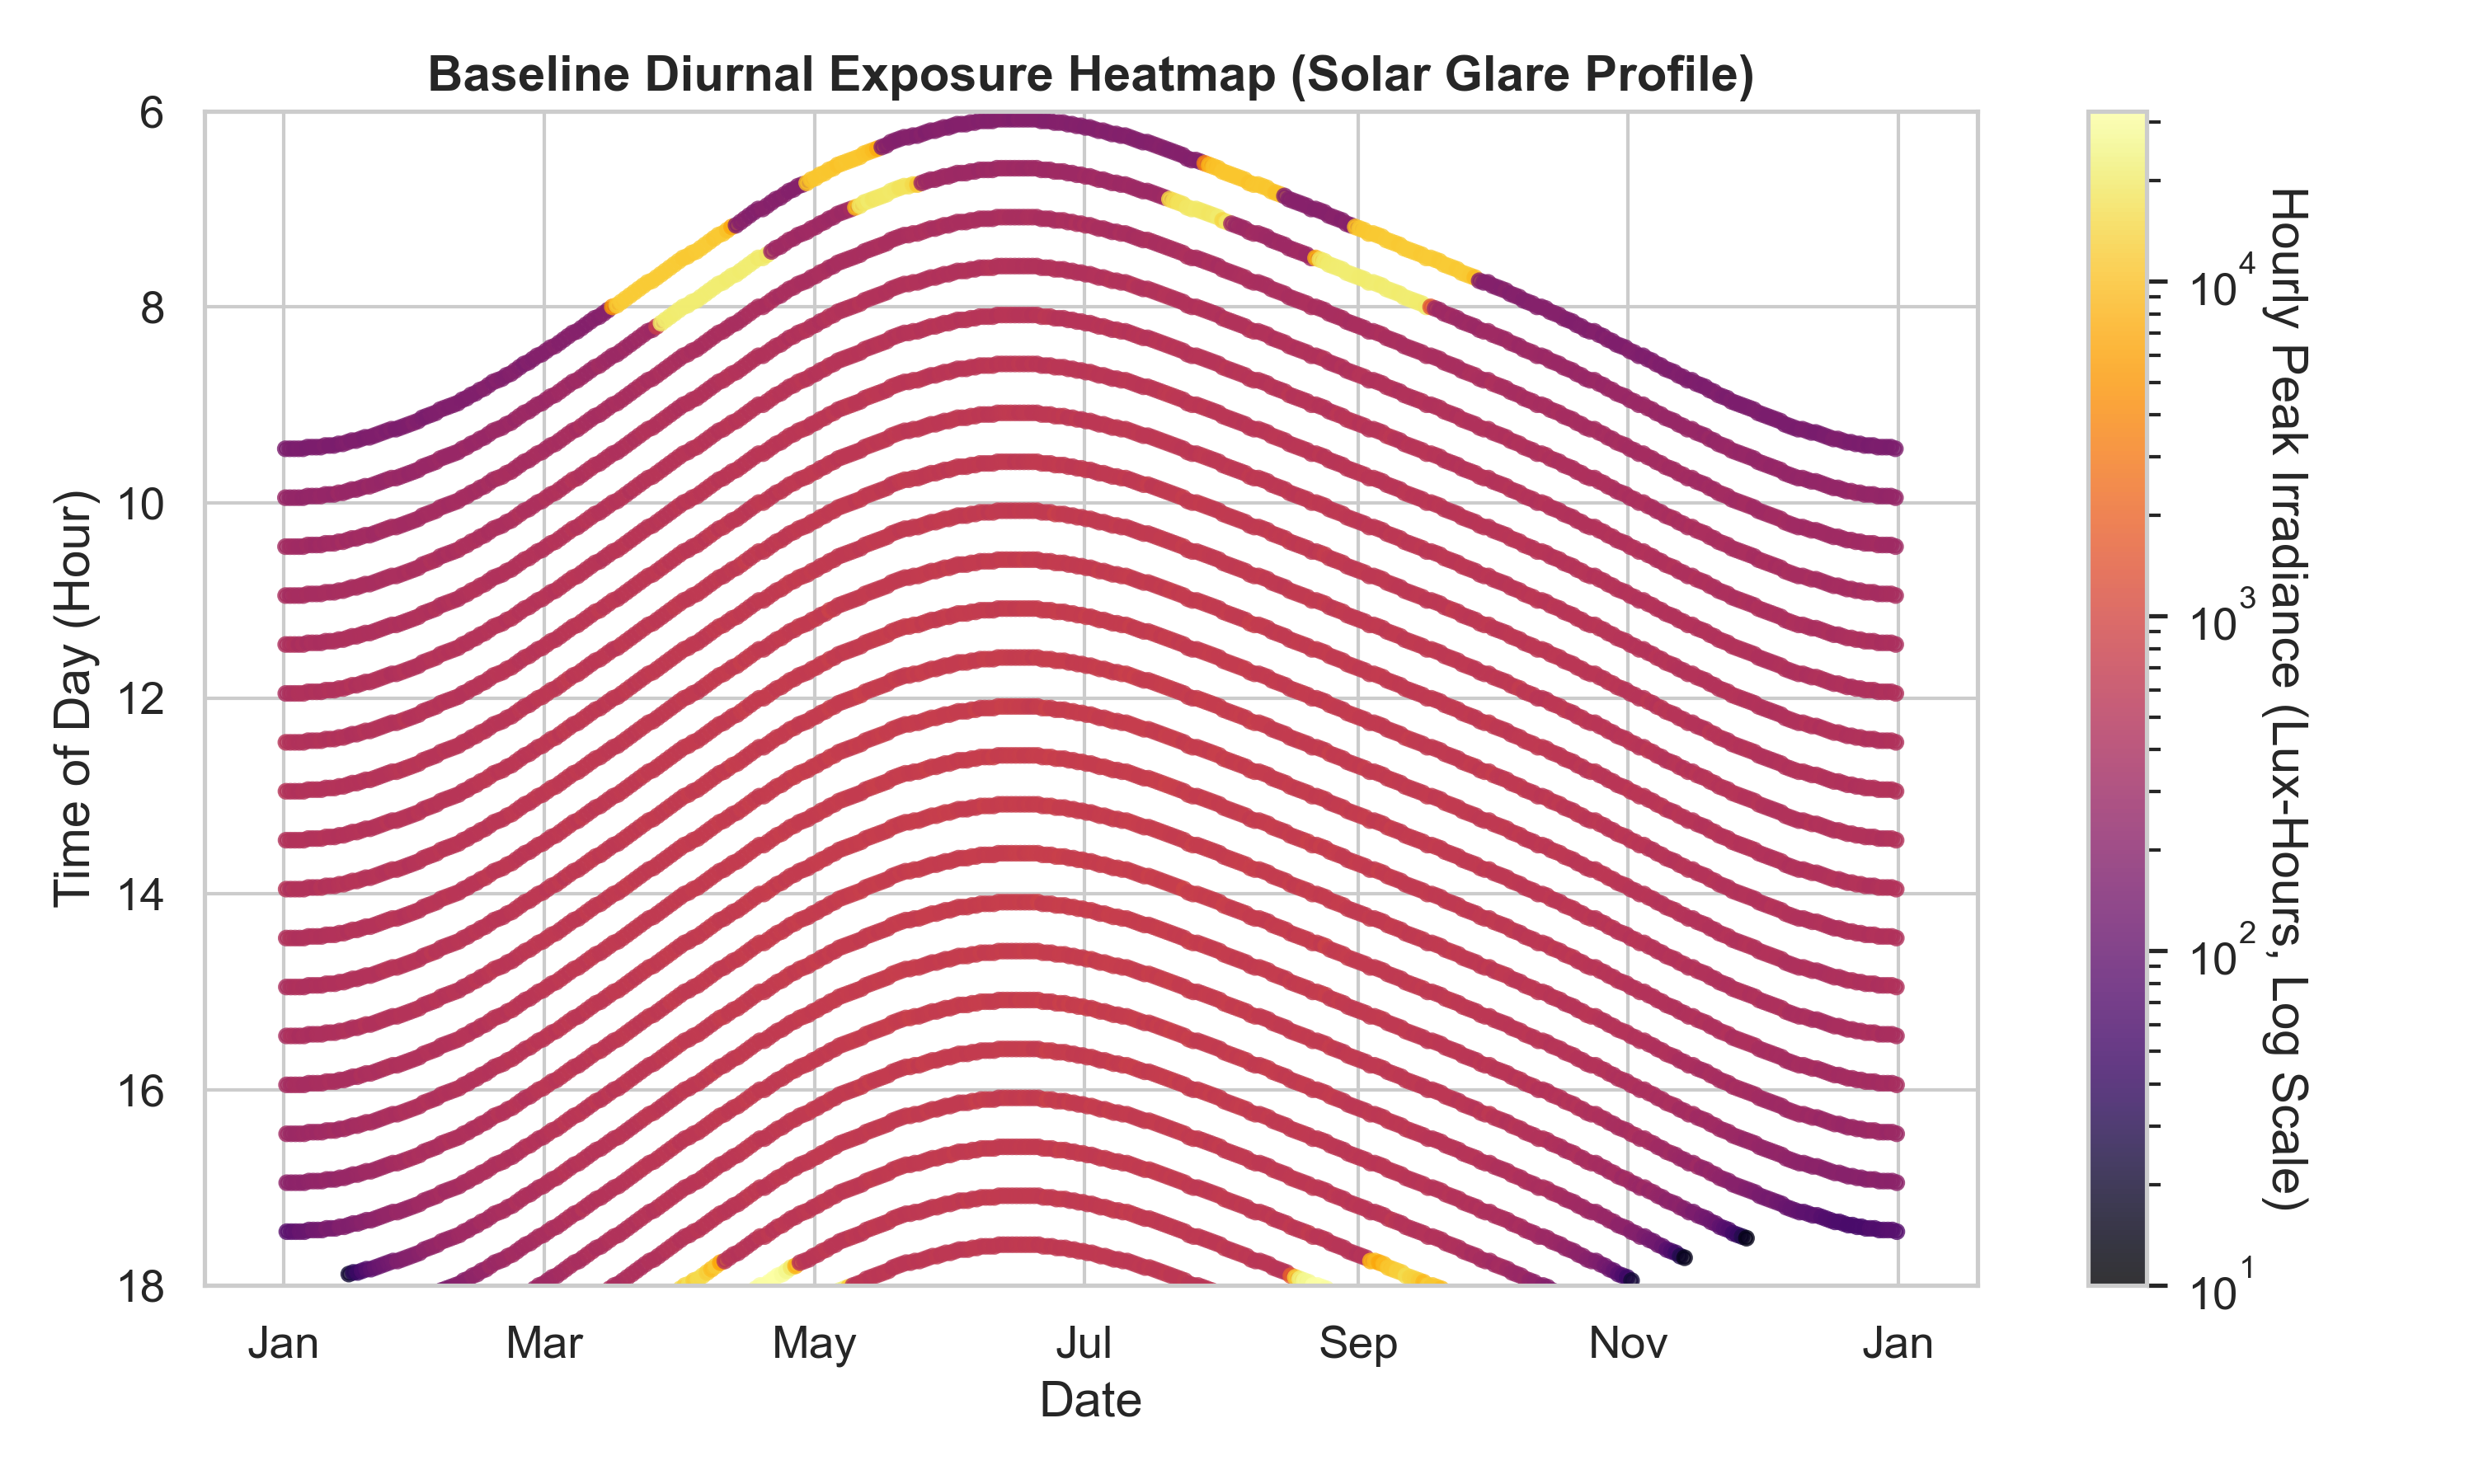
\includegraphics[width=0.9\columnwidth]{fig4_diurnal_heatmap.png}}
    \caption{A heat map of diurnal exposure illustrates hourly exposure levels in 365-day cycle, displaying high frequency peaks corresponding to solar noon hours and seasonal solar elevation changes.}
    \label{fig:scenario_a_diurnal}
\end{figure}

The plot shown in Figure~\ref{fig:scenario_a_diurnal} visualizes the diurnal variation in illumination levels. Note the spikes of intensity at solar noon time and changes at solstice periods in June/December, highlighting the necessity of computation of a full meteorological year in order to calculate a precise diurnal profile rather than using static offline lightmaps.

\subsection{Scenarios B, C, and D: Conservation Interventions}
In order to test the ability of our preventative conservation measures, we took advantage of the interactive features of our Digital Twin and performed a comparative study of 3 scenarios against our baseline setup A. Scenario B (Material Intervention) involves changing the environmental setup, but keeping the original position of the asset. It includes replacing the window glass with conservation tinted glass that blocks UV radiation (transmittance $T = 0.45$, albedo $R = 0.12$) and reducing the amount of reflected ambient light by making the floor material matte ($R = 0.15$). Scenario C (Positional Optimization) explores the effects of geometric occlusion, the asset was placed in a shaded corner of the room. The architectural materials were restored to their initial highly reflective state. Lastly, Scenario D (Combined Intervention) explores the interaction of changing the location and adding protective glass and floor materials.

\begin{figure}[htbp]
    \centerline{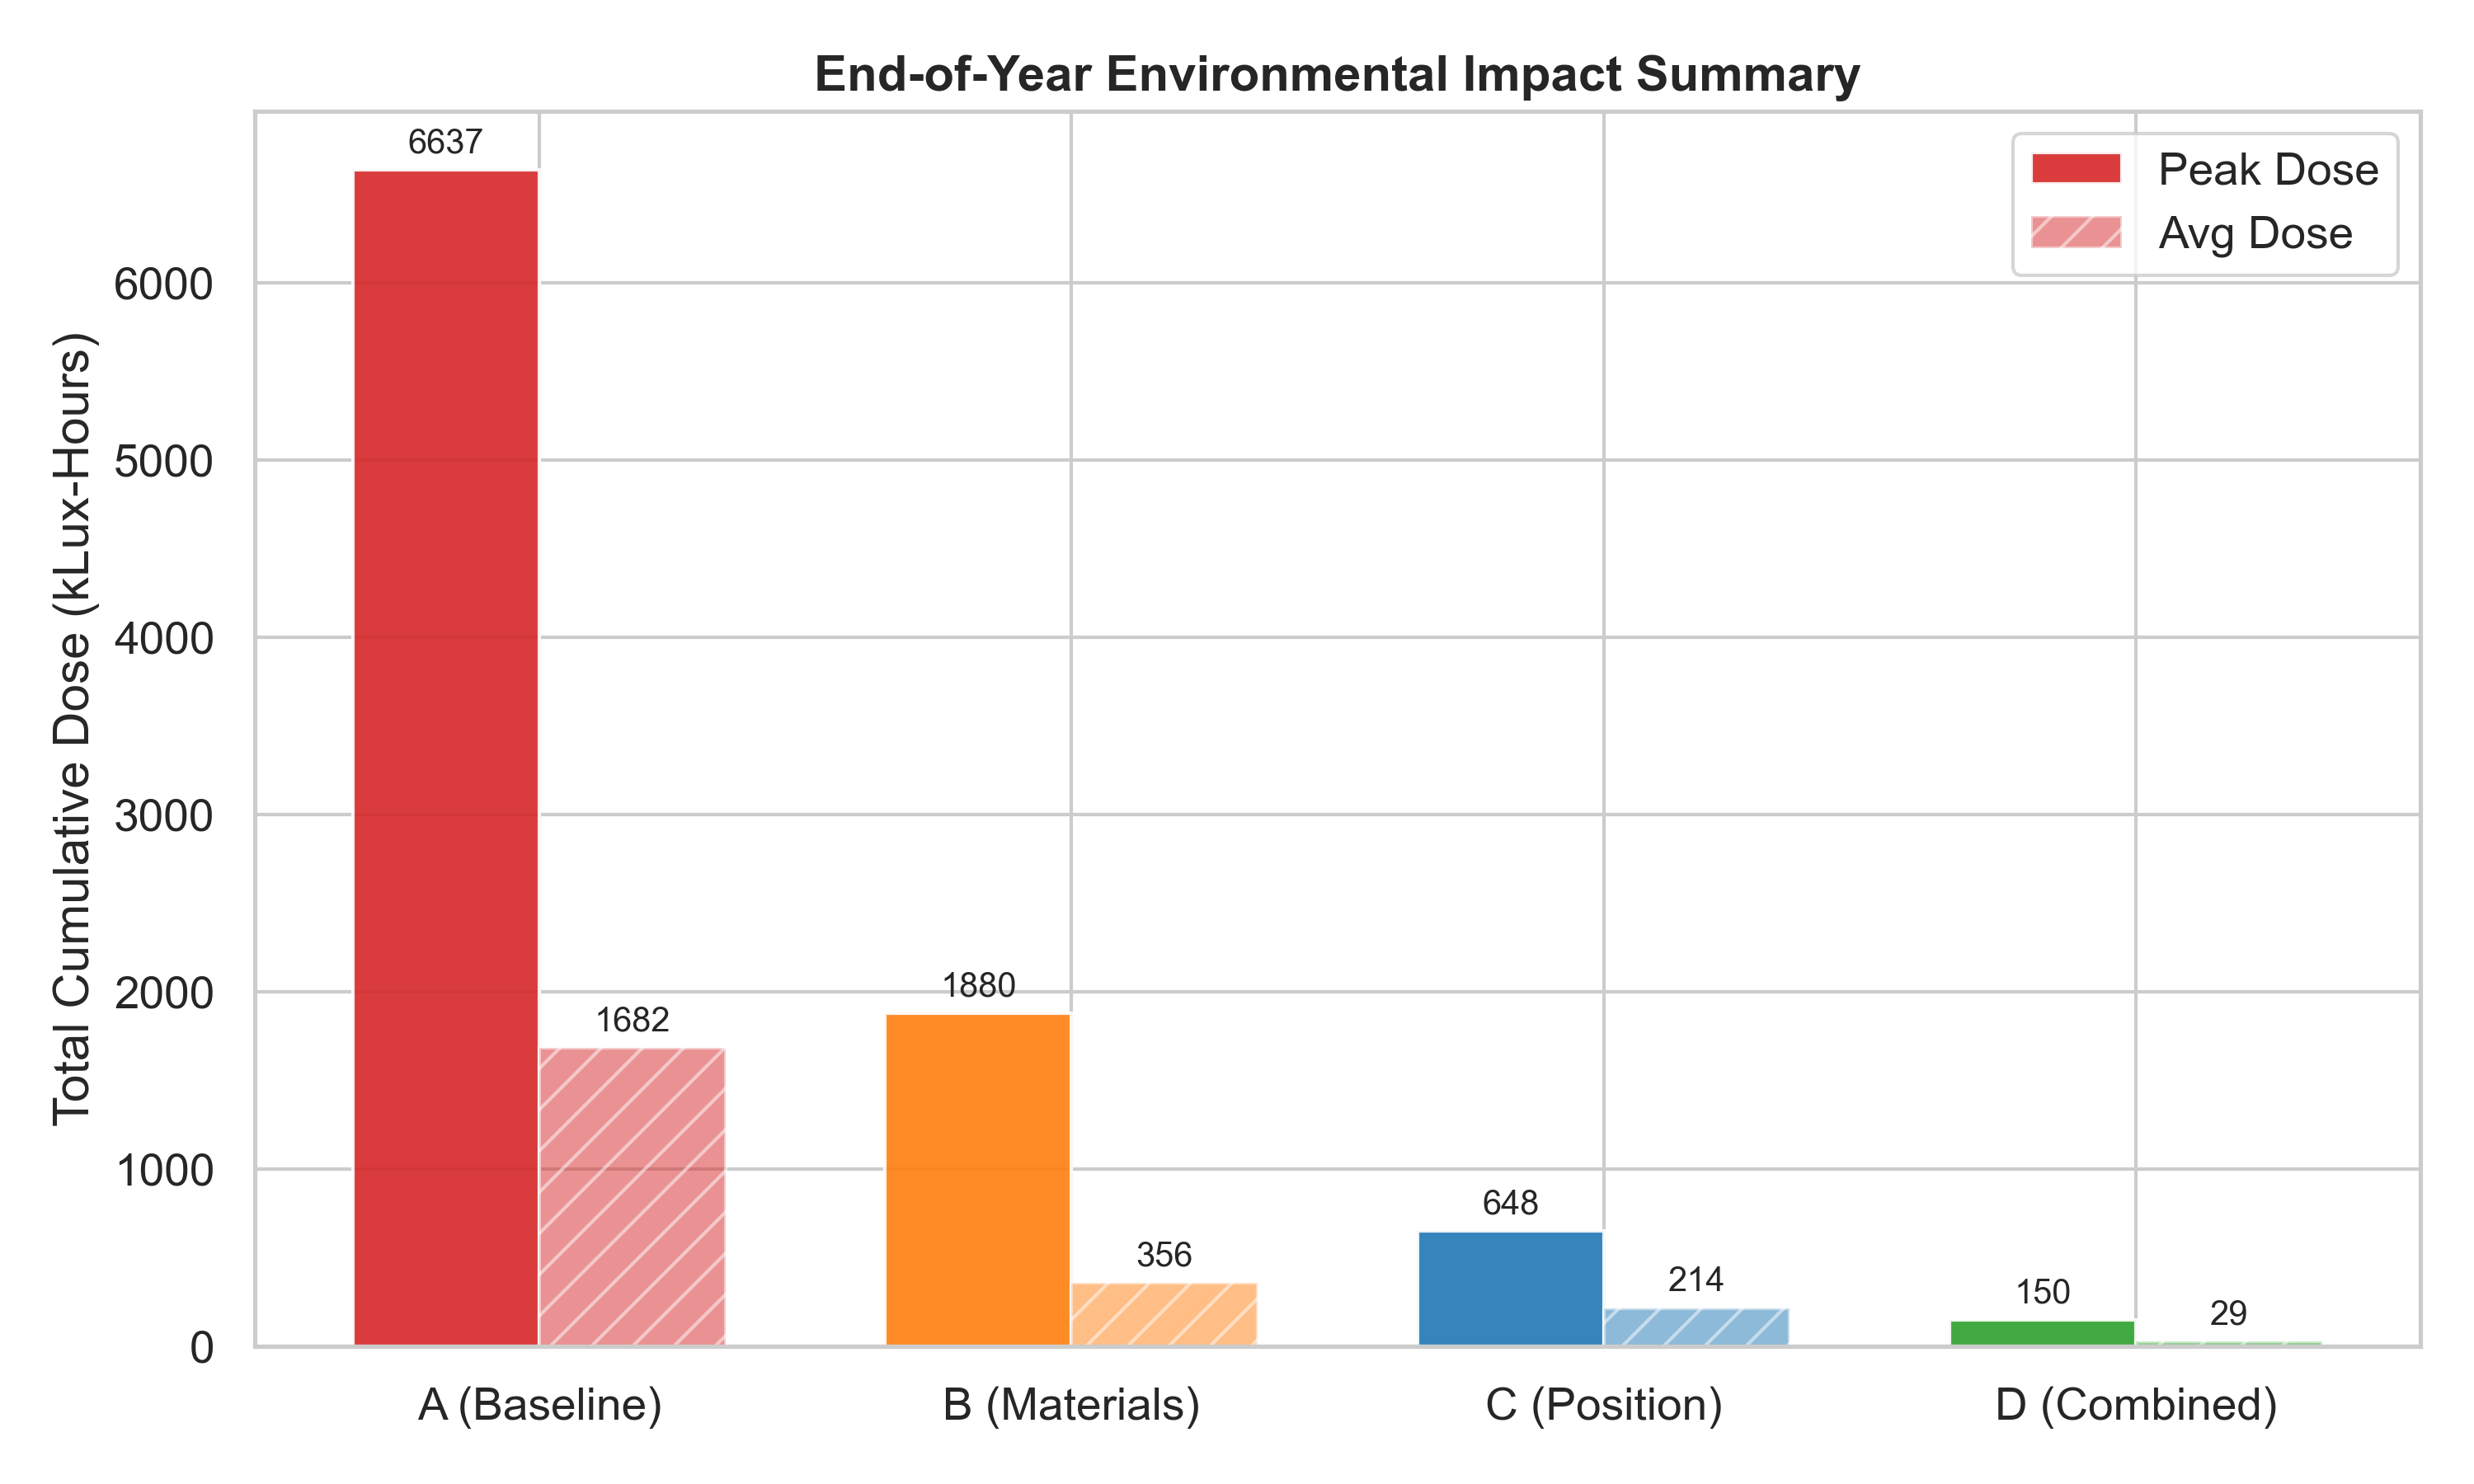
\includegraphics[width=0.9\columnwidth]{fig2_final_dose_bar.png}}
    \caption{Comparative study of peak light dose in four scenarios illustrates the effectiveness of Scenario D that combines optimization of the asset location with implementation of the protective materials.}
    \label{fig:scenario_comparative_bar}
\end{figure}

The telemetry results shown in Figure~\ref{fig:scenario_comparative_bar} demonstrate a substantial reduction in light dosimetry in all three proposed scenarios compared to the baseline of 6.6M Lux-Hours. Scenario B reduces the peak light dose to 150k Lux-Hours, while Scenario D provides the best overall metrological protection.

These results illustrate the usefulness of our Digital Twin for simulating and validating synergistic conservation architectural retrofits without incurring real costs and risk associated with actual physical renovation projects.

\subsection{Phenomenological Analysis: Window vs. Corner Geometry}
An analysis over a span of 10 days during the winter solstice was carried out to demonstrate the capabilities of the Digital Twin regarding modeling non-traditional geometries in daylighting (Figure~\ref{fig:window_vs_corner}). This study involved comparing peak hourly doses for artifacts placed next to the window and those of artifacts placed deep in a room corner.

\begin{figure}[htbp]
    \centerline{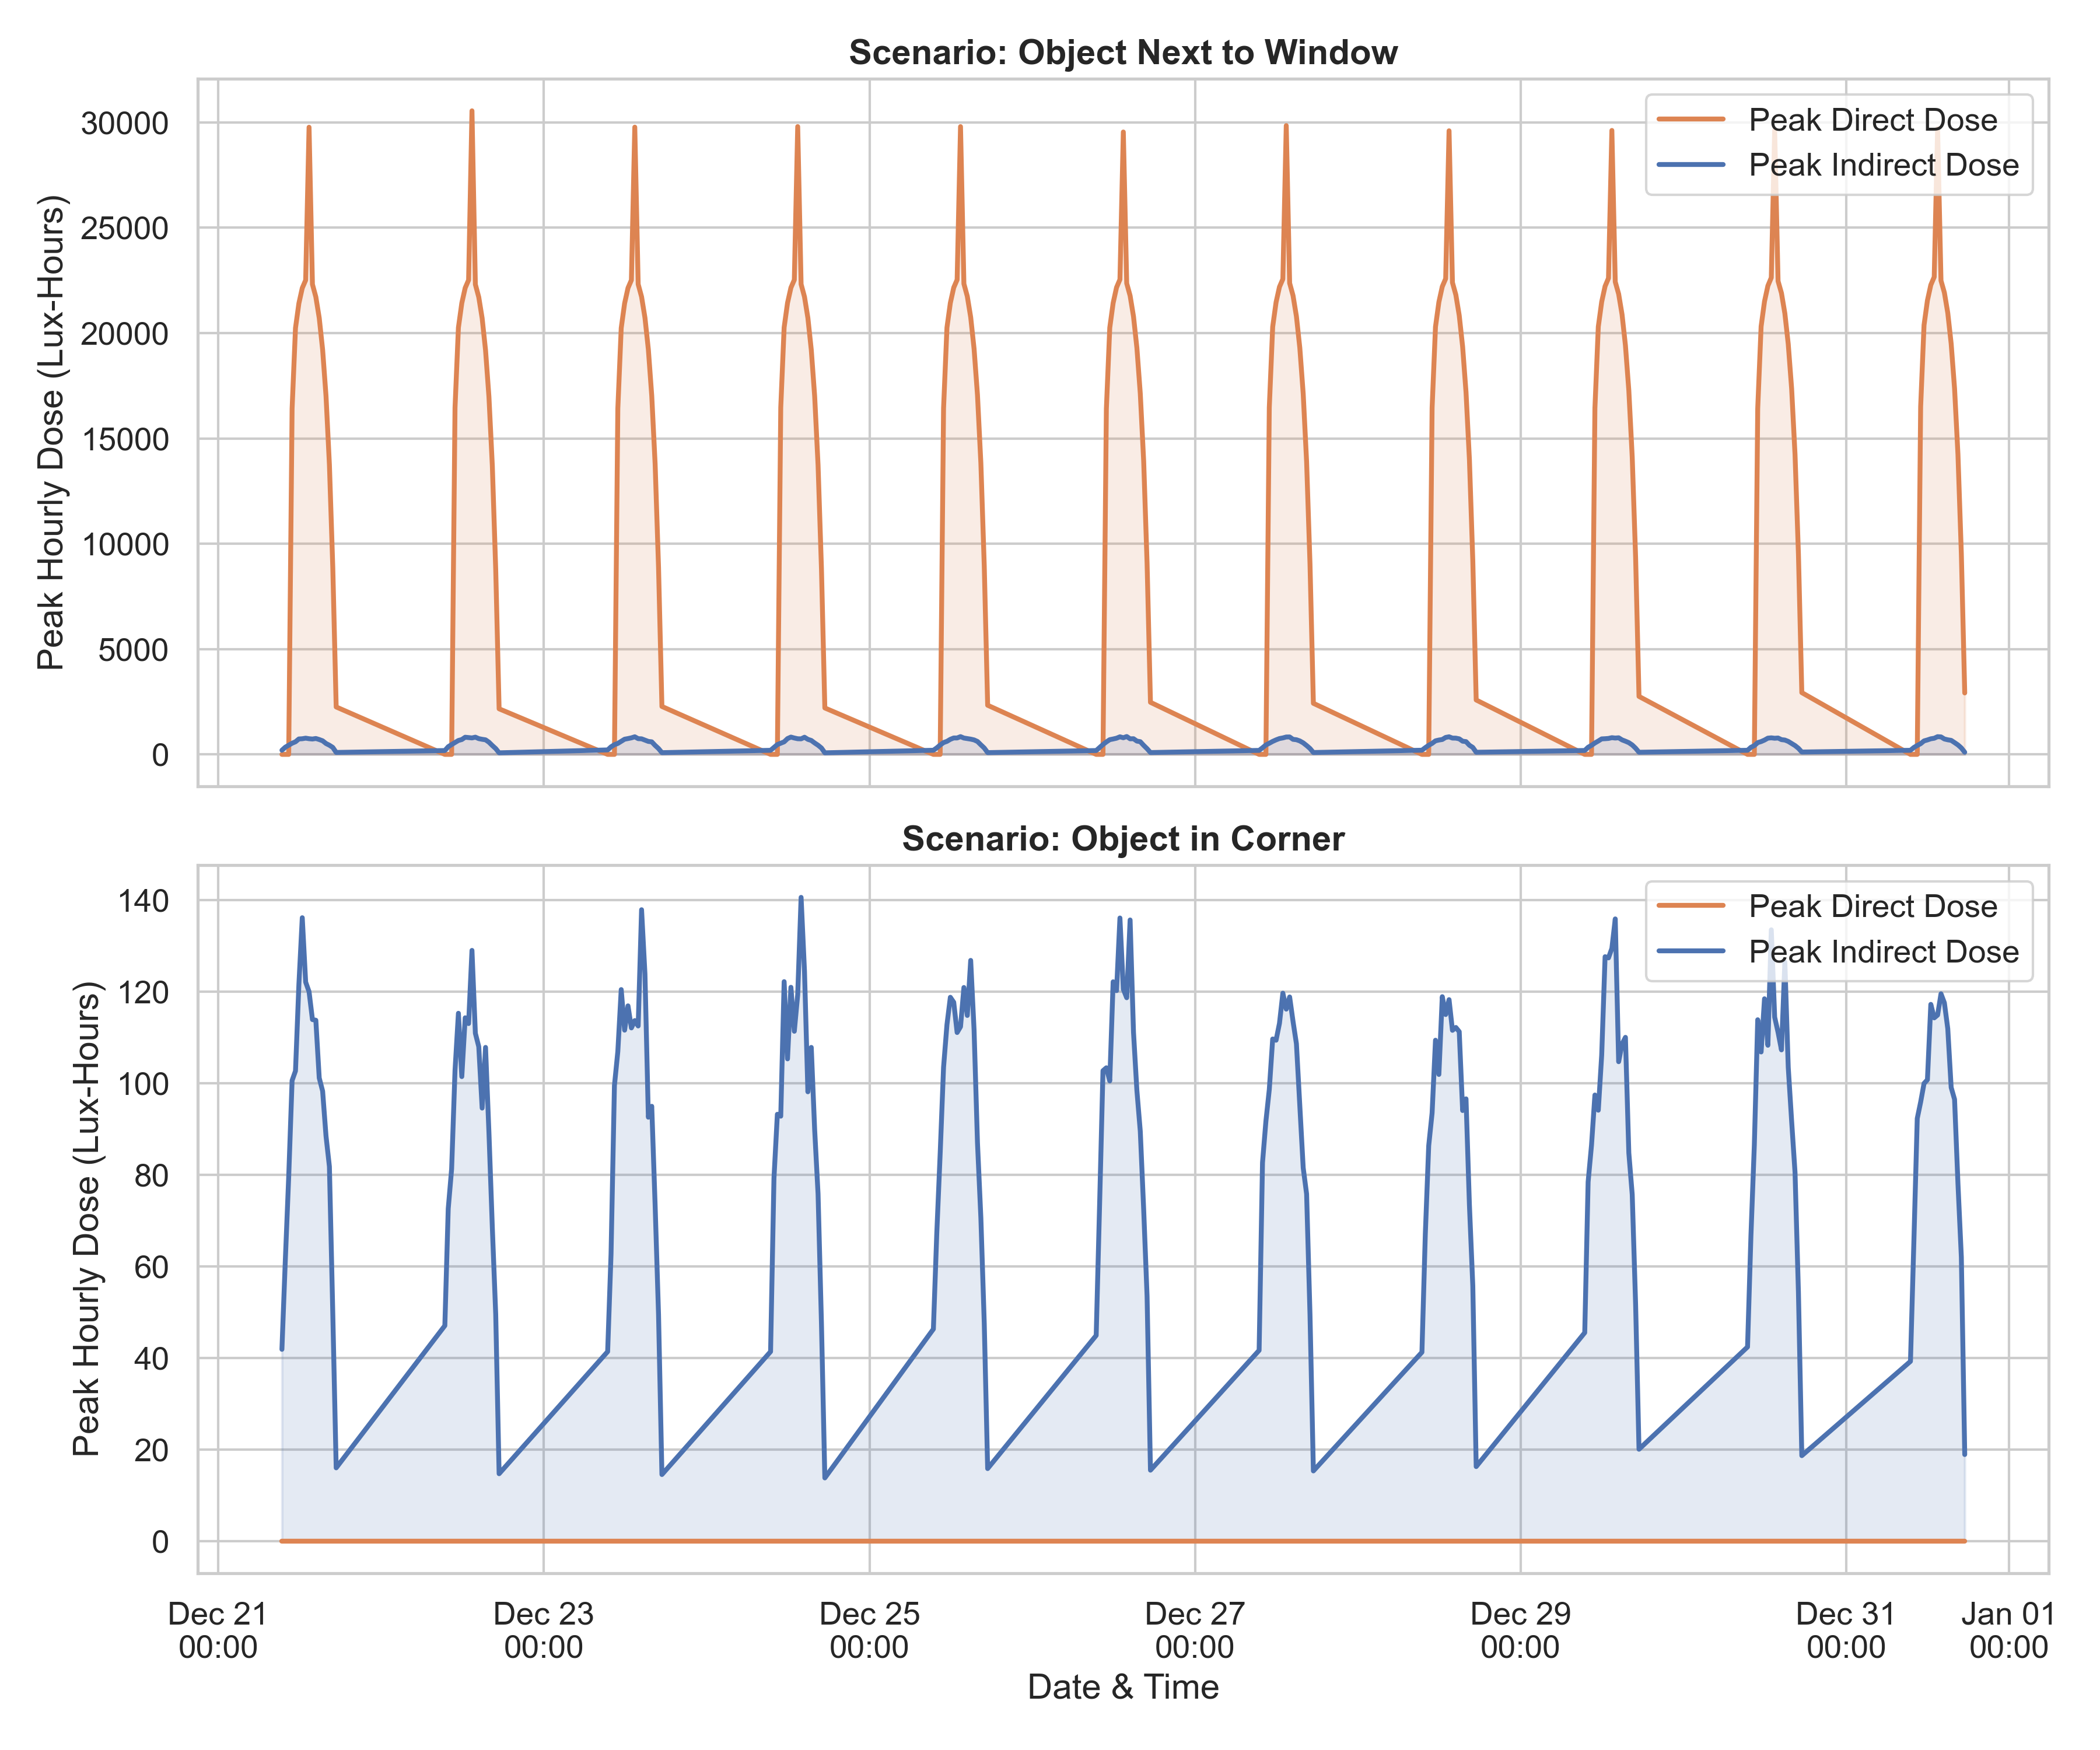
\includegraphics[width=0.9\columnwidth]{fig6_window_vs_corner_comparison.png}}
    \caption{The 10 day winter solstice comparison of peak hourly doses for artifacts placed next to windows with artifacts placed deep in room corners is presented. As seen from the empirical results below, the case with artifacts placed next to the window is dominated by a large direct solar component, while no direct sunlight falls on the second type of artifacts and the light dose is exclusively determined by the indirect and diffuse ambient contribution.}
    \label{fig:window_vs_corner}
\end{figure}

The data demonstrates the dynamic nature of daylighting geometry with respect to the winter solstice. Artifacts placed next to the window experience large direct sunlight concentrations reaching 30,000 Lux-Hours and largely exceeding any indirect ambient exposures. In the case of artifacts placed inside the room corner, the direct solar contribution is completely blocked by the architecture, resulting in a zero dose from this source. Hence, the indirect dose makes up 100\% of the total exposure and is caused by scattered light from the sky. This conclusively proves the simulator's capability to correctly compute complex cosine-weighted hemispherical irradiance and physical shadowing without resorting to approximations.

\section{Performance \& Validation}

\subsection{Computational Efficiency}
Texture space ray-tracing paradigm offers numerous performance benefits. Traditional CPU-based offline rendering of light stress typically takes several hours for one chronological exposure. Our framework is based on the DX12 engine and uses GPU hardware acceleration of intersection cores to achieve real-time interactivity. Calculation of telemetry data is performed asynchronously, and the rendering process operates at constant stable 60 FPS rate.

\subsection{Scientific Validation}
Though the process of heat maps generation requires minor computational effort, metrological analysis requires us to make sure about the accuracy of calculations from a physical standpoint. Hence, the necessity to automatically place the Lux sensors outside the scene and analyze their spatial variance ($\sigma^2$) as well as convergence errors arose. The entire procedure took place during 8,760 rendering cycles of the scene.

The sensors in question are capable of sampling raw, untone-mapped floating point telemetry data taken from GPU accumulation buffers asynchronously. They are automatically positioned outside the scene bounds; hence, the irradiance measured at those locations can be used for the comparison with theoretical results based on the cited formulas. Convergence error of the Monte Carlo simulation is evaluated via $SEM = \sigma / \sqrt{N}$ formula, where $SEM$ stands for standard error of the mean. It should be noted that $\sigma$ is sample standard deviation while $N$ equals the number of rays sampled per pixel. As weather simulation integrates with the program, the error gradually decreases to zero.

\begin{figure}[htbp]
    \centerline{
\includegraphics[width=0.9\columnwidth]{fig3a_spatial_dose_variance.png}}
    \caption{Continuous monitoring of light spatial variance tracking aggregated structural stress on the artifact.}
    \label{fig:validation_stress_variance}
\end{figure}

\begin{figure}[htbp]
    \centerline{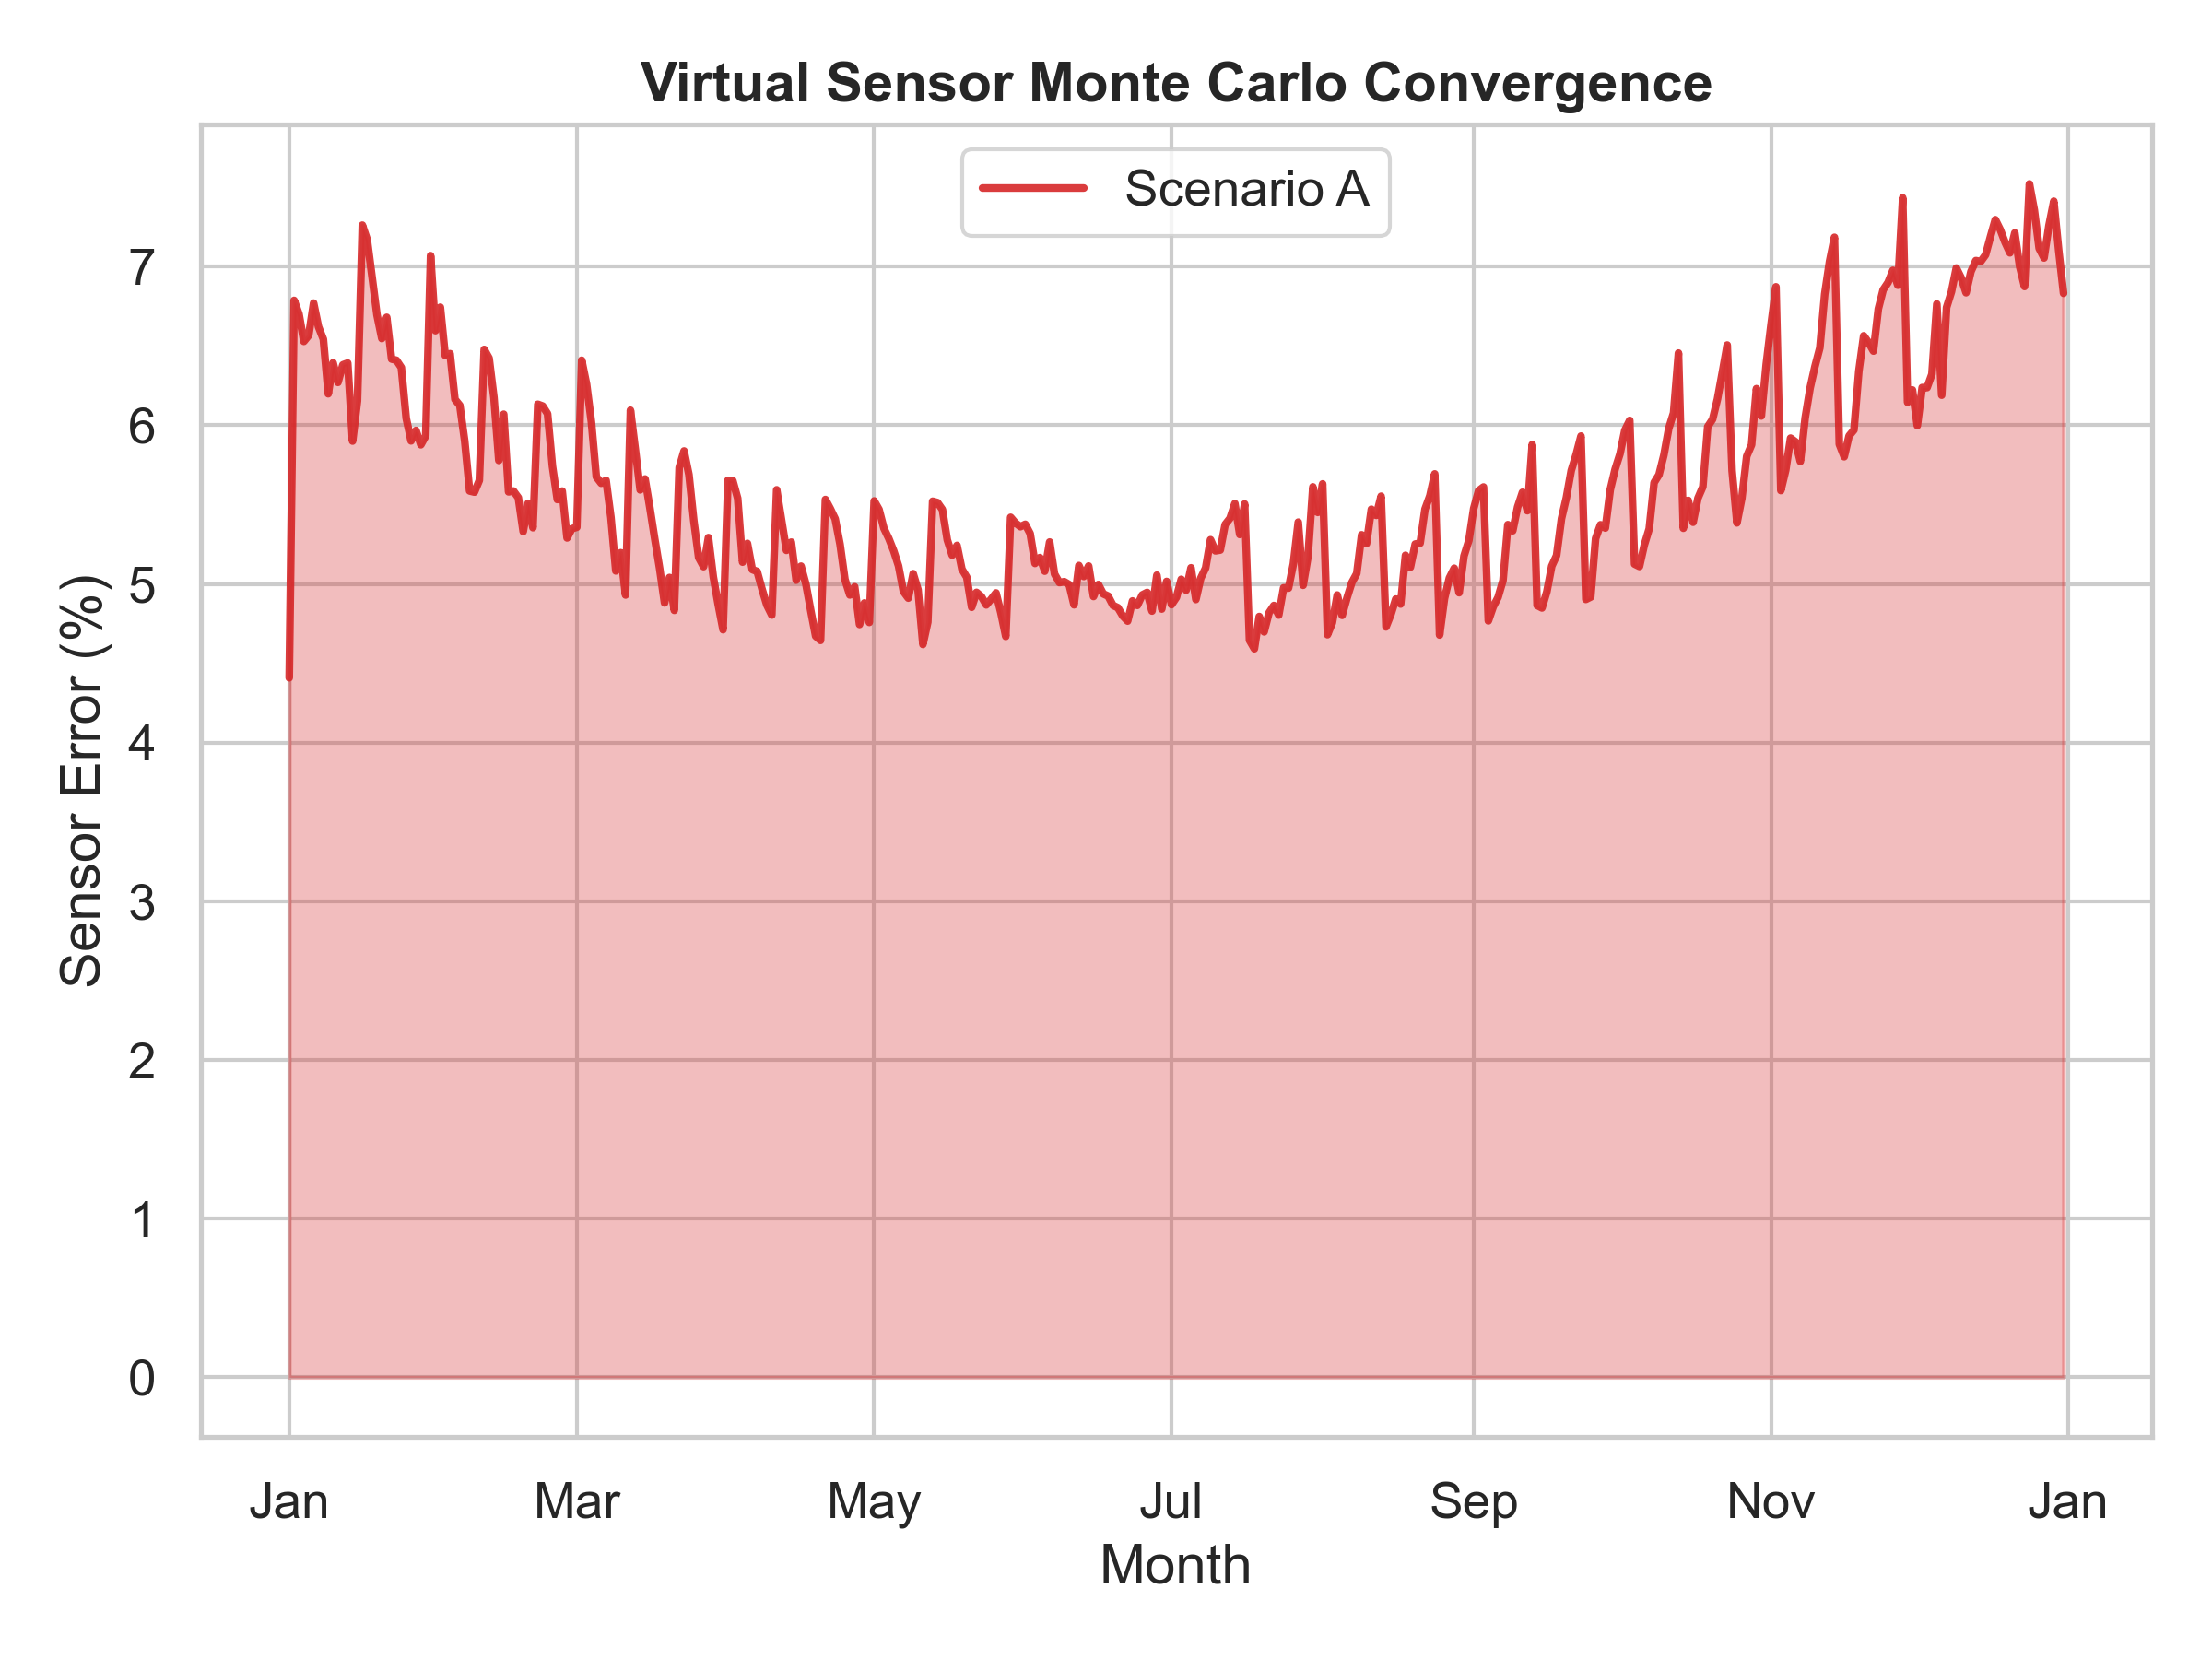
\includegraphics[width=0.9\columnwidth]{fig3b_monte_carlo_convergence.png}}
    \caption{Virtual Sensor Monte Carlo convergence error confirms stable convergence and validates our GPU-based calculation pipeline.}
    \label{fig:validation_stress_error}
\end{figure}

The graphs provided in Figure~\ref{fig:validation_stress_variance} and Figure~\ref{fig:validation_stress_error} prove that Monte Carlo convergence error steadily drops and stabilizes during the calculation process. Spatial variance converges with the physical light stress accumulation rather than noise generated by the Monte Carlo algorithm, thereby proving the reliability of the GPU-based integration and allowing export of physically accurate CSV arrays.

In addition, the noted differences in terms of shape among the variance curves can be directly attributed to the placement of the artifact and its related incidence angle toward the sun. The peaks that have been noted in certain periods are directly correlated to the time periods when the direction of the vector from the sun is able to give it an uninterrupted path to the artifact, hence causing variance in the radiation levels. Despite these notable changes based on seasons and geometry, it is evident that the general trend of the curves still holds strong. Mathematically speaking, it shows the correctness of the Monte Carlo engine.



\section{Conclusion \& Future Work}
This paper presented ChronoLux, an interactive, hardware-accelerated Digital Twin framework explicitly engineered for the scientific metrology of photodegradation in cultural heritage artifacts. By fundamentally rethinking the rendering pipeline and shifting from transient screen-space rasterization to permanent Texture Space Ray Tracing, we successfully solved the temporal and spatial limitations that previously restricted graphics engines from performing rigorous radiometric dosimetry.

Through the integration of the Perez All-Weather Sky Model and a highly optimized DirectX 12 Monte Carlo path tracer featuring Next Event Estimation (NEE), ChronoLux demonstrated the capability to continuously integrate 8760 hourly solar intervals within a stable, interactive 60 FPS viewport. This represents a monumental leap in computational efficiency, compressing what traditionally required hours of offline, CPU-bound rendering into a real-time, exploratory tool.

The empirical case studies validated the framework's efficacy as a non-destructive conservation sandbox. By simulating the long-term light exposure of a 2K high-fidelity Stanford Bunny scan, we demonstrated how the Digital Twin can isolate and quantify the exact radiometric impact of varying environmental interventions. Scenario testing revealed that synergistic interventions---such as repositioning the artifact to exploit geometric occlusion alongside the installation of UV-blocking tinted glazing and matte flooring---could successfully reduce a catastrophic 6.6 million Lux-Hour peak dose down to safe conservation thresholds of less than 150k Lux-Hours. Most critically, the scientific metrology was mathematically validated. By utilizing an automated array of out-of-bounds virtual Lux Sensors to sample the raw, untonemapped accumulation buffers, we tracked the Monte Carlo convergence error via the standard error of the mean ($SEM = \sigma / \sqrt{N}$). The continuous integration proved that the variance graphs structurally adhere to the physical realities of shifting solar vectors, confirming that the engine reliably calculates stable, physically-based light transport dynamics rather than stochastic rendering noise.

\subsection{Future Work}
Despite having the ability to provide an accurate mathematical basis for geometric and radiometric metrology of fading in objects at present, there is much room for growth in the field, which can take place via a number of approaches.

Firstly, the most essential mathematical enhancement in the current version will be the inclusion of material-specific spectral sensitivity curves. Presently, the program uniformly integrates raw radiometric irradiance values. In future versions, however, the framework should be upgraded to accommodate internal floating-point representation and incorporate CIE $V(\lambda)$ luminous efficiency curve as well as ISO Blue Wool standard fading spectrums. With the introduction of wavelength-dependent spectral arrays that go beyond broadband radiometry, the framework would have the ability to make highly accurate predictions about colorimetric fading ($\Delta E$) and material degradation rate, e.g., differentiating between that of 16th-century oil paints and that of acrylic.

Secondly, there are many benefits to the framework incorporating the option of dynamic architectural loading. The framework presently uses a static pre-compiled model of the scene. With further developments to the C\# engine, it would become possible for museum curators and architects to use an OBJ or glTF file parser to load entire new models of buildings into the simulation engine dynamically. This way, the program would be able to act as a truly universal tool for museums or heritage sites across the world, requiring no initial setup or pre-compilation in the Unity Editor beforehand.

Lastly, the ability of the framework to predict fading rates can be localized by integrating live or historical meteorological APIs. Presently, the program uses a static sky with a worst-case Perez model of irradiance with $T = 2.0$. With the help of a REST API connection to local meteorological stations with historical data, the program would be able to build an accurate digital twin of the weather and atmospheric state, making it possible to accurately emulate irradiation based on historical values of the aerosol optical depth and atmospheric pressure in particular geographic locations.

Additionally, the modern dependency on high-performance consumer graphics cards in architecture makes both financial and technological entry barriers for small conservation laboratories. It is reasonable and beneficial to consider a logical next step in the development of the ChronoLux system -- adopting a distributed cloud rendering technology infrastructure. Using remote computing for running complex DirectX 12 Compute Shader computations and Monte Carlo ray-tracing engine will allow the simulation results to be accessed by multiple thin clients simultaneously through cloud technology infrastructure that includes an enterprise-grade GPU-equipped data center. Thus, it is possible to make this expensive piece of equipment unnecessary for the operation of the program by switching to cloud infrastructure.

\bibliographystyle{IEEEtran}
\bibliography{references}

\end{document}
